\let\negmedspace\undefined
\let\negthickspace\undefined
\documentclass[journal]{IEEEtran}
\usepackage[a5paper, margin=10mm, onecolumn]{geometry}
%\usepackage{lmodern} % Ensure lmodern is loaded for pdflatex
\usepackage{tfrupee} % Include tfrupee package

\setlength{\headheight}{1cm} % Set the height of the header box
\setlength{\headsep}{0mm}     % Set the distance between the header box and the top of the text

\usepackage{gvv-book}
\usepackage{gvv}
\usepackage{cite}
\usepackage{amsmath,amssymb,amsfonts,amsthm}
\usepackage{algorithmic}
\usepackage{graphicx}
\usepackage{textcomp}
\usepackage{xcolor}
\usepackage{txfonts}
\usepackage{listings}
\usepackage{enumitem}
\usepackage{mathtools}
\usepackage{gensymb}
\usepackage{comment}
\usepackage[breaklinks=true]{hyperref}
\usepackage{tkz-euclide} 
\usepackage{listings}
% \usepackage{gvv}                                        
\def\inputGnumericTable{}                                 
\usepackage[latin1]{inputenc}                                
\usepackage{color}                                            
\usepackage{array}                                            
\usepackage{longtable}                                       
\usepackage{calc}                                             
\usepackage{multirow}                                         
\usepackage{hhline}                                           
\usepackage{ifthen}                                           
\usepackage{lscape}
\begin{document}

\bibliographystyle{IEEEtran}
\vspace{3cm}
\title{1.1.9.7}
\author{EE24BTECH11032 - John Bobby}
% \maketitle
% \newpage
{\let\newpage\relax\maketitle}

\renewcommand{\thefigure}{\theenumi}
\renewcommand{\thetable}{\theenumi}
\setlength{\intextsep}{10pt} % Space between text and floats


\numberwithin{equation}{enumi}
\numberwithin{figure}{enumi}
\renewcommand{\thetable}{\theenumi}

\textbf{Question:}The distance of the point $(-6,8)$ from the orgin is

\solution The length of a vector is defined as\\
\begin{align}
	\left\lVert x \right\rVert &= \sqrt{x^Tx}\\
	x &=\myvec{-6\\8} \\
	x^Tx &=\myvec{-6, 8}\myvec{-6\\8} = 100\\
	\left\lVert x \right\rVert &= \sqrt{100}=10
\end{align}
Thus the distance of the point $(6,-8)$ from the orgin is $10$ units.
\begin{figure}[h!]
                \centering
               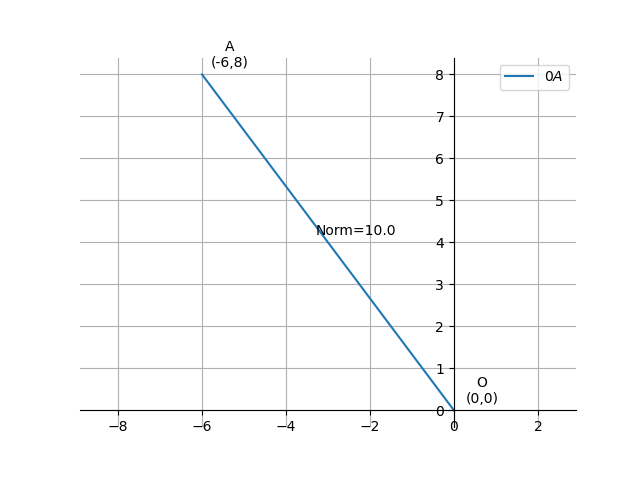
\includegraphics[width=0.7\linewidth]{Figs/Fig1.png}
			\caption{Plot of point $(6,-8)$}
               \label{stemplot}
               \end{figure}
\end{document}

